\documentclass{article} % Määritellään luotavan dokumentin tyyppi

\usepackage{amsmath} % Matematiikkapaketti

\usepackage{amsfonts}

\usepackage[utf8]{inputenc} % UTF-8 merkistö

\usepackage[T1]{fontenc} % Tuki ääkkösille

\usepackage{parskip} % Rivinvaihto kappaleiden väliin, ei sisennystä

\usepackage{graphicx} % Grafiikkapaketti kuvien lisäämiseen

\usepackage{epstopdf} % Mahdollisuus lisätä *.eps tyyppisiä kuvia

\usepackage{verbatim}

\usepackage{float}

\usepackage{pdfpages}


\title{ELEC-A7150 - C++ Programming \\Game Implementation: Micro Machines \\ mmachines2}
\date{\today}
\author{Arto Lehisto \\ Sampsa Hyvämäki \\ Tuomas Poutanen \\ Mikko Murhu\\}


\begin{document}

\maketitle

\newpage

\tableofcontents

\newpage

\section{Overview}

The outcome of the project is a driving game mimicking the style of Micro Machines. The game has a local split-screen two player mode, in which the players compete to finish a set number of laps first. The players have to avoid obstacles while trying their best to disturb their opponent’s driving by shooting at him. Launching the game lets the user access the menu. From the menu, the user can change settings or start a game at a specific map. There are multiple maps to choose from and implementing more isn’t difficult. Figures \ref{mainMenu}, \ref{keySetup}, \ref{keySelect}, \ref{mapSelect} and \ref{mapNot} show the views the user sees when navigating in the menu. Figure \ref{ingame} shows the in-game view.

\begin{figure}[H]
\centering
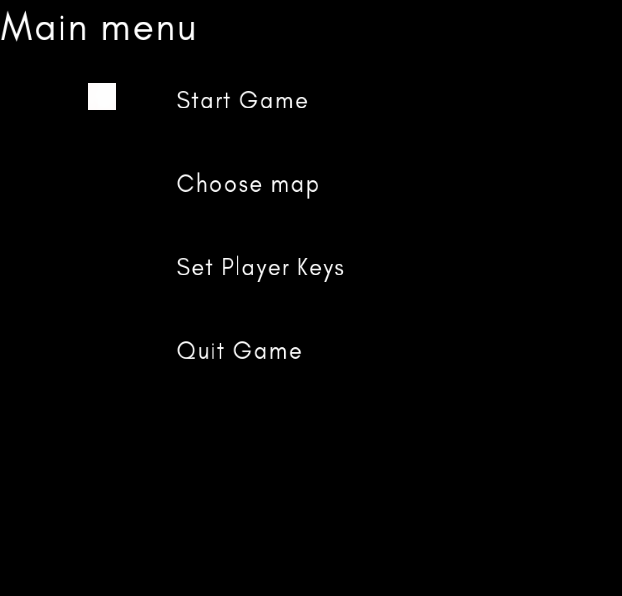
\includegraphics[width=120mm]{images/mainmenu}
\caption{View of the main menu.}
\label{mainMenu}
\end{figure}  

\begin{figure}[H]
\centering
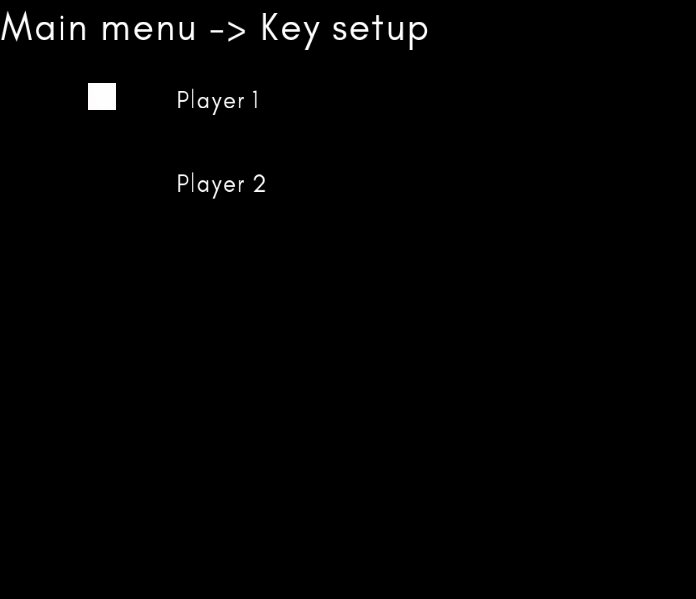
\includegraphics[width=120mm]{images/key_setup}
\caption{View of the key setup menu.}
\label{keySetup}
\end{figure}  

\begin{figure}[H]
\centering
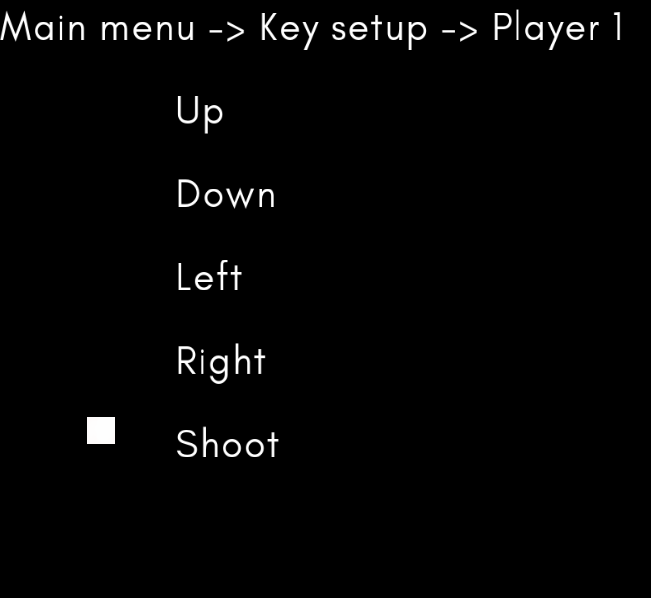
\includegraphics[width=120mm]{images/key_select}
\caption{View of the key setup menu, when setting keys.}
\label{keySelect}
\end{figure}  

\begin{figure}[H]
\centering
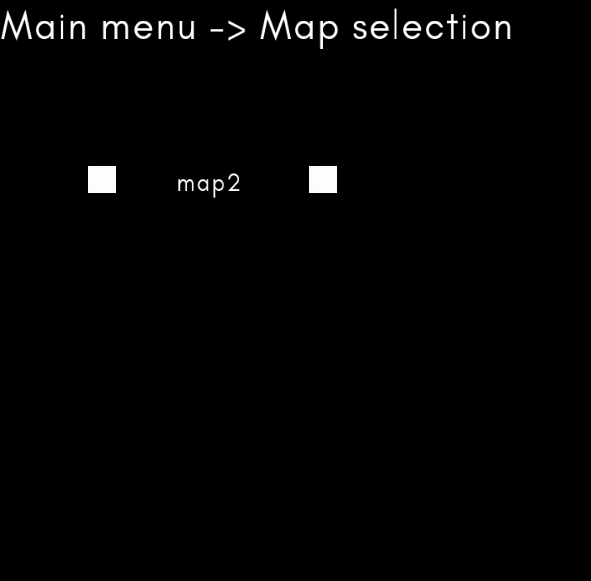
\includegraphics[width=120mm]{images/map_s_selected}
\caption{View of the map selection menu. The selection is indicated by the white square on the right-hand-side.}
\label{mapSelect}
\end{figure}  

\begin{figure}[H]
\centering
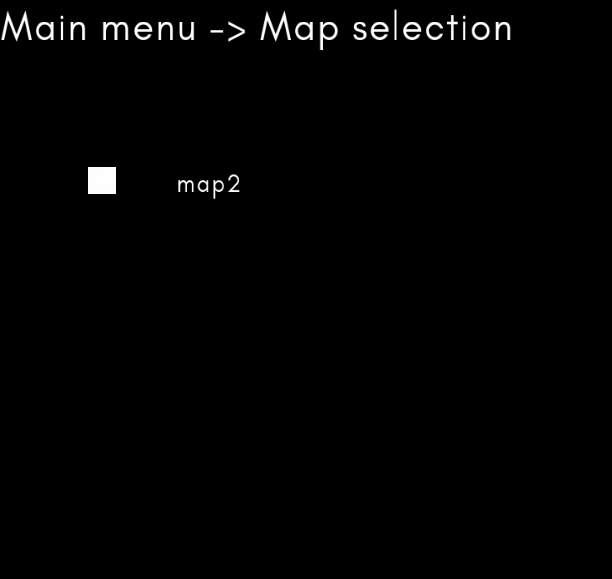
\includegraphics[width=120mm]{images/map_selection_not_selected}
\caption{View of the map selection menu. There is no white square next to the map now, so this is not the selected map.}
\label{mapNot}
\end{figure}  

\begin{figure}[H]
\centering
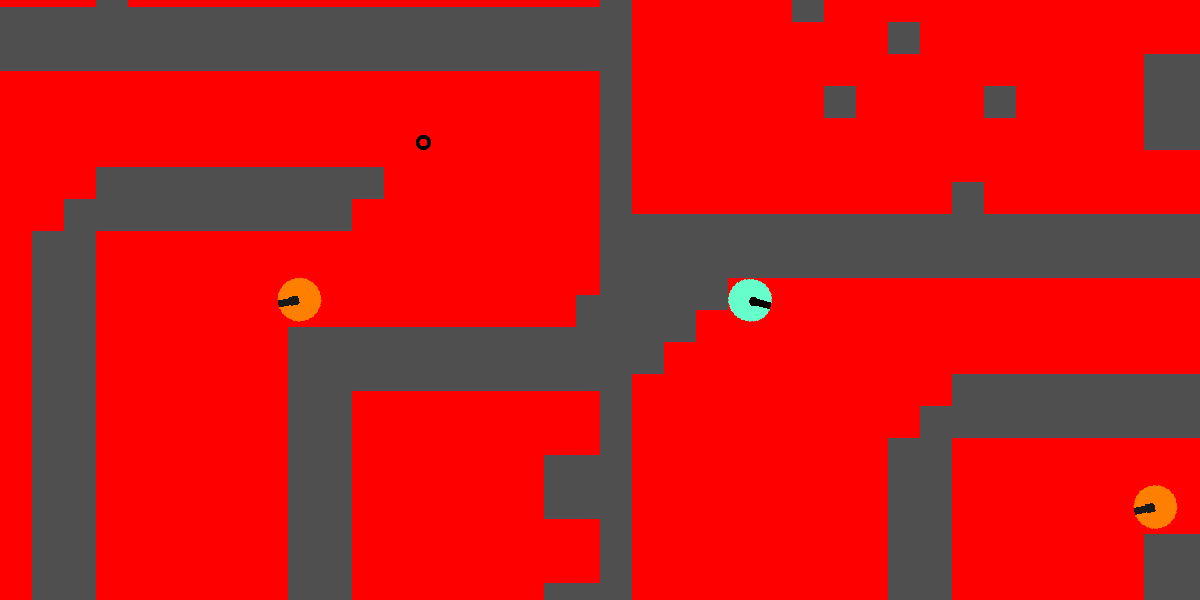
\includegraphics[width=120mm]{images/splitscreen}
\caption{View of the in-game screen. The users control one of the circles that their splitscreen views follow.}
\label{ingame}
\end{figure} 

\section{Software structure}
Among with standard C++11-libraries, the software uses SFML (simple and fast multimedia library) for creating a graphical user interface typical for a computer game: while running, the program handles screens, in which the user can define game setting or play the game. The program flow consists of changing back and forth between the screens until the user decides to exit the game. The program is implemented using object-oriented programming: inside the main-function, class instances are created and the values of their member variables are changed by calling their member functions. During the game development, a class structure described in figure \ref{uml} was created.

\begin{figure}[H]
\centering
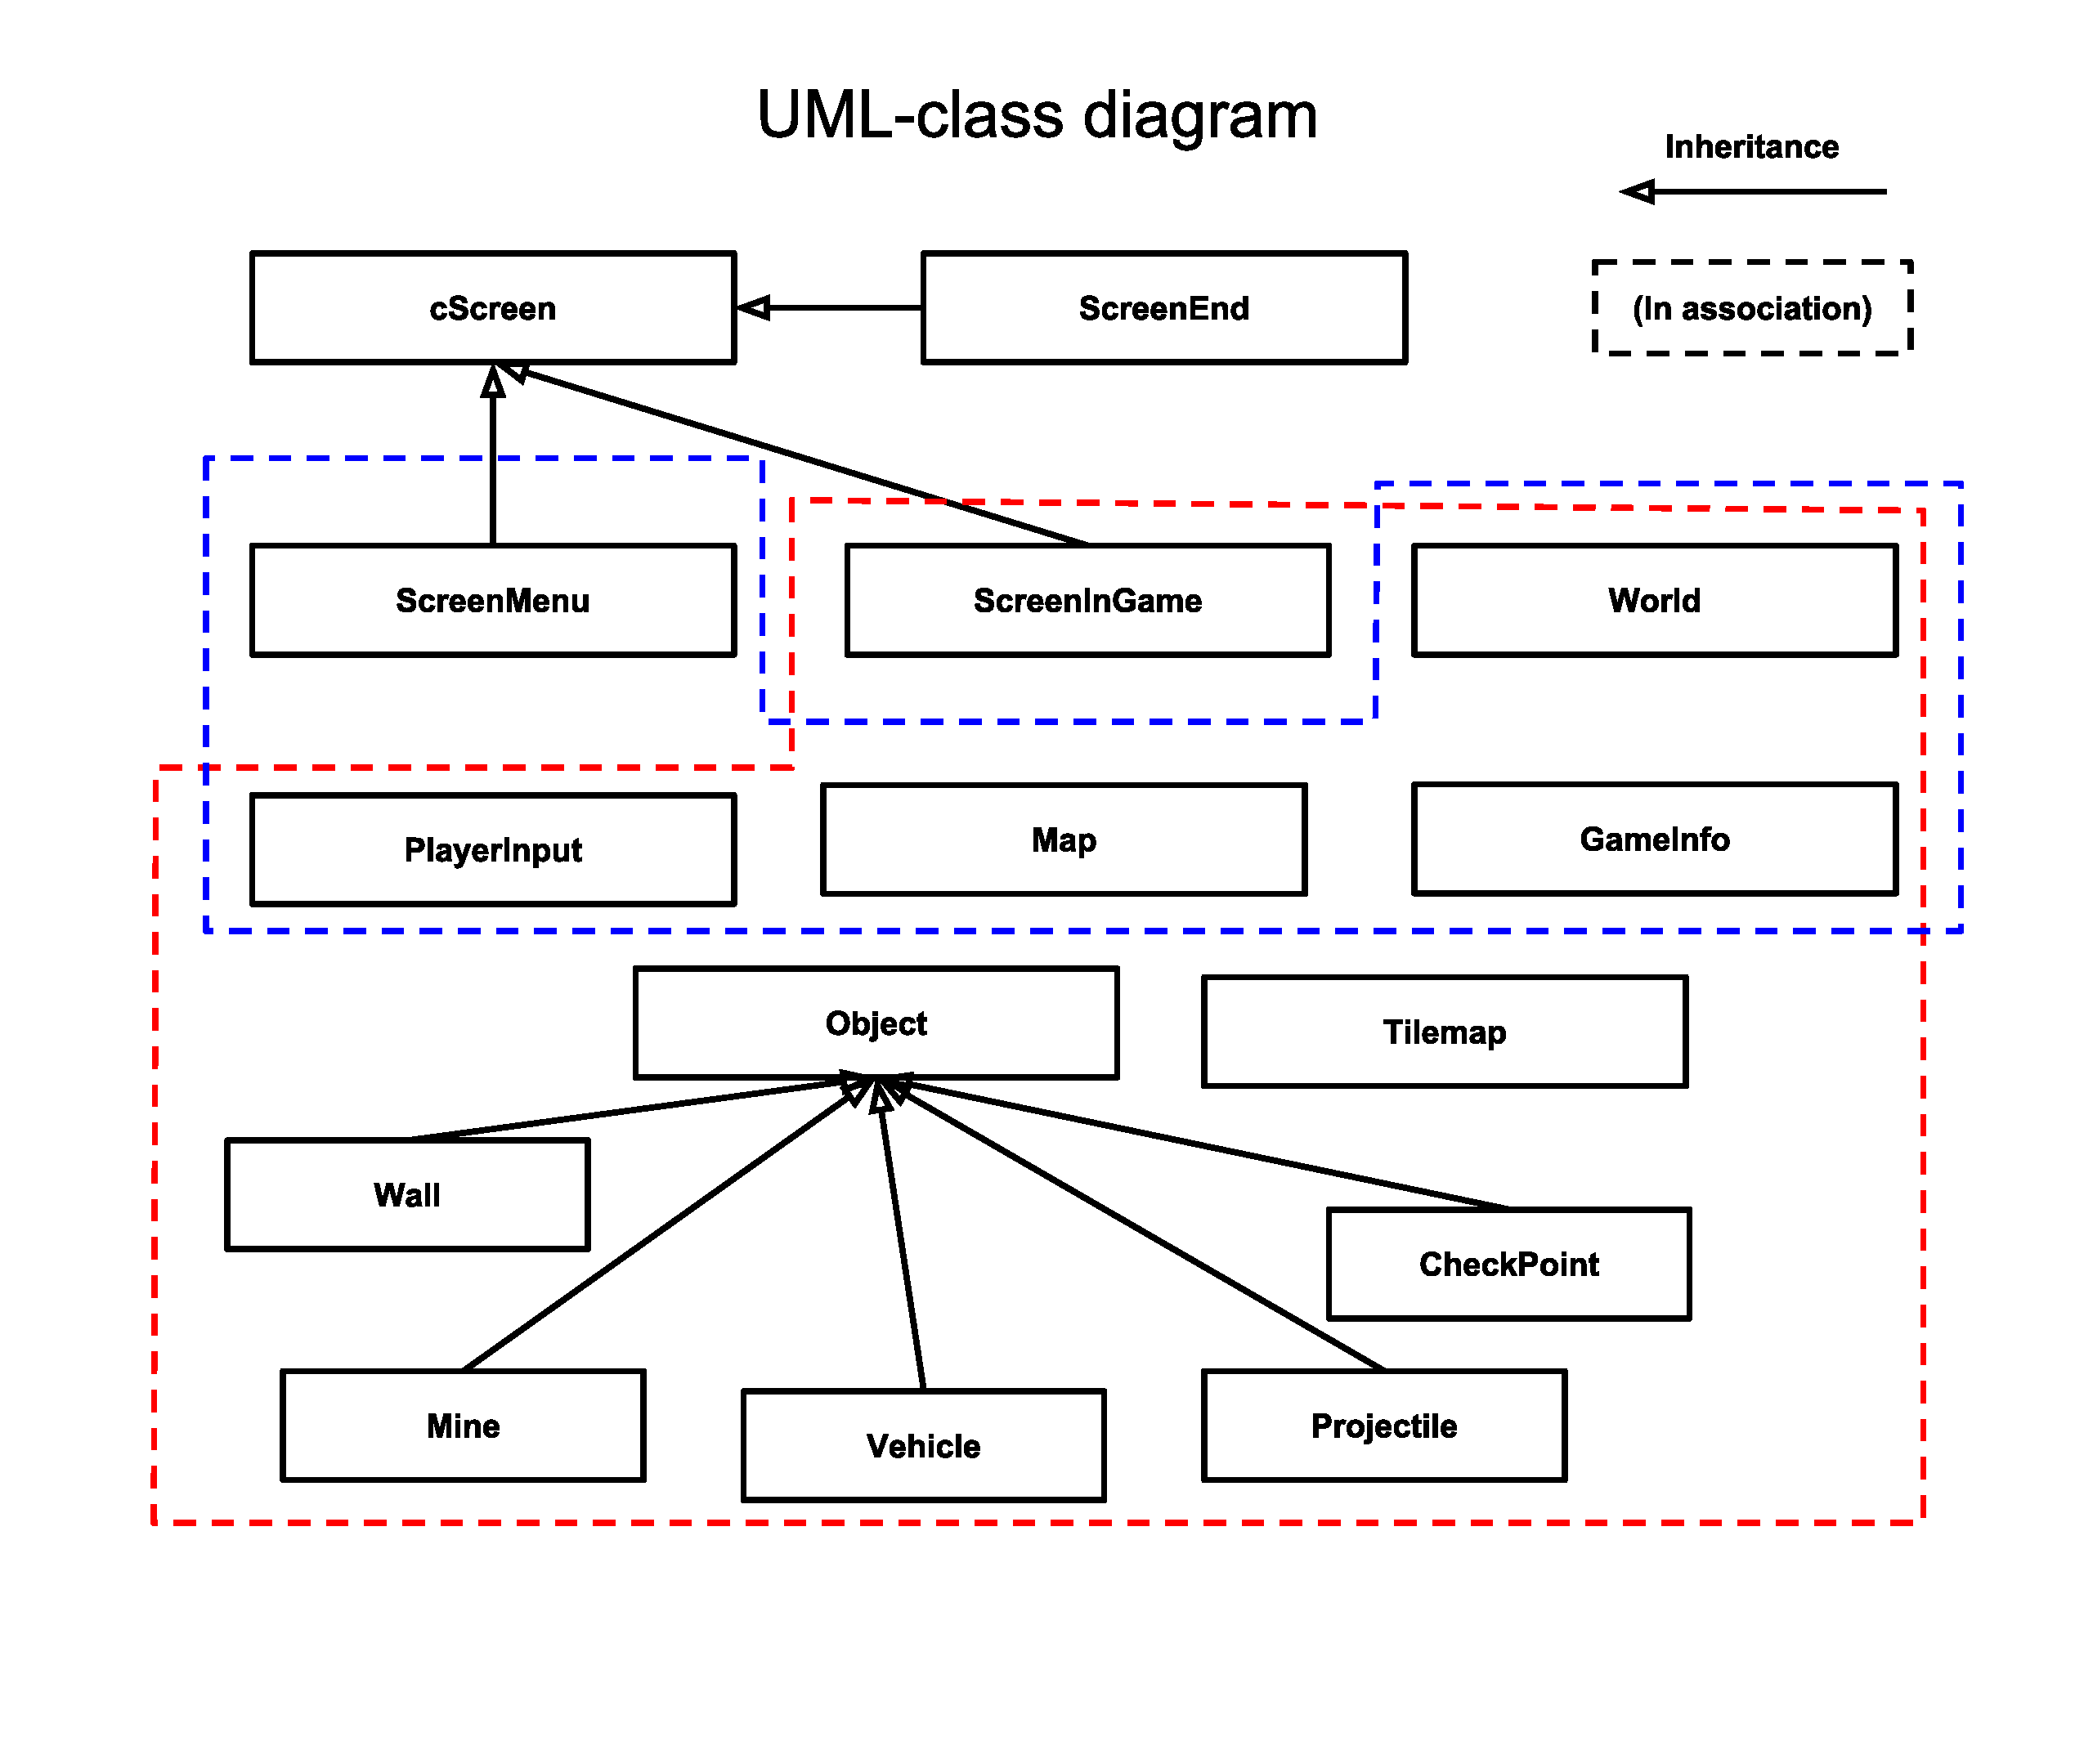
\includegraphics[width=120mm]{images/uml}
\caption{The UML-class diagram of the project.}
\label{uml}
\end{figure}  

\section{Description of software logic}
The game consists of drawable items that move according to user-input and collide resulting in different reactions. The main loop calls for different screens for different game stages. The screens implement while-loops that render the game and in the in-game screen update the status of drawables.

Preserving game data and running relevant checks of collisions and game logic etc. is performed in an instance of the World class. The game map is read from a textfile including locations of walls and checkpoints and parameters of vehicles and mines. The map on the background is created only once in the form of a tilemap class, which is lighter to render than tiles on their own. When the text file is read, map, walls, checkpoints, mines and vehicle parameters are saved in the world instance. Two player class instances are created for controlling player input. The game is ready to start: for each rendered frame multiple physics updates are performed. Each physics update updates the state of the world; that is, location of projectiles and vehicles, the state of game obstacles, collisions etc. 

All collidable items are inherited from the base class Object.  The Object-class contains methods that are used by all game objects, such as those linked to collision detection and object rendering.


In addition to the actual gameplay, there are two stages of the game. In the menu, user can define game-settings (choose a map and set input keys) and in the endscreen, player is informed of completing the game. As mentioned before, these stages are implemented by using the screen-class. The class-instance itself has only one member function (Run), which contains instructions to run that stage of the game and, most importantly, draw things to a window given to it as a function parameter. The return value of the function defines the next game stage and indicates the closing of the program. Screen has one member variable, pointer to GameInfo-object which stores important information that is accessible to every screen (e.g. chosen map).

\section{Instructions for building and using}

We use make for building our project. In order to build the project, one must have make installed on their system. After that one can build and run our project by typing “make run” into a terminal that is in the project’s root directory. This builds the project and starts the application.
The application consists of two main parts: A main menu and the actual game. The user can navigate in the menu using arrow keys. Up and down arrow keys change the option that would be selected, right arrow key selects the option and left arrow key returns to the previous menu. To select a map, choose the “Choose map” option and scroll through the maps using up and down arrow keys, then select the map with the right arrow key. The selected map will be indicated by a white square to the right-hand-side of the map. After the preferred map is selected, the user can start the game by selecting “Start game” on the top menu.

In game, the user can move using the arrow keys for player 1 and wasd for player 2, by default. Player 1 shoots with space and player 2 shoots with tab. These inputs can be changed in the settings. The user can also press escape to return to the menu. 

To quit the game, choose “Quit Game” in the top menu. 

\section{Testing}

In the beginning, testing was done purely by compiling the project to make sure there is nothing wrong with the syntax. We built a main function quite early, and after that we could also test the application by running it. This kind of testing was mostly done by two methods, by printing something to the standard output to see a glimpse of individual behavior of some function and by taking notice on what happens on the game window and deducting something from that behavior. In case of memory leaks, we used valgrind to find out the offending piece of code.

\section{Work log}

Week 45: The first implementation of makefile, planning of the project started

Arto: Implemented the makefile, tinkered with git file filtering (8h)\\
Sampsa: (4 hrs)\\
Tuomas: Some practice on makefiles (4 hrs) \\
Mikko: (4 hrs)\\

Week 46: Project plan was created together

Sampsa: Began the implementation of Map-class, created a function to read the data from textfile to the program memory (8 hrs)\\
Tuomas: Created a class for Tiles with enumeration for tiletype and function, which later proved to be useless. Watched and read lots of tutorials regarding creating games with sfml (5h)\\
Arto: Worked on the tile class, worked on the object class (5h)\\
Mikko: Worked on basic physics, Object-class and Vehicle-class. (6h)\\

Week 47: 

Sampsa: Finished a first working version of map-class, the program could now get the name of the map, tiletypes, dimensions and map matrix from a textfile. Made also first testmaps. (10 hrs)\\
Tuomas: Learned how to draw tiles. Added basic graphs for tiles to be drawn and figured out how to present the routes for graphics. Had some issues with the scope of the program, since the graph route is different depending on from which context the program is run. (5h)\\
Arto: Added a Player (later renamed to PlayerInput) class for handling player input. Found out with other team members that separate tiles are way too resource intensive to implement our map properly. Implemented a tilemap class based on sfml’s vertex arrays to alleviate this. Moved function implementations from map header file to map code file. (10h)\\
Mikko: Continued implementing physics, the Object-class and the Vehicle-class. (4h)\\

Week 48:

Sampsa: In a refresher training (military) from 26.11. to 5.12. (0 hrs)\\
Tuomas: Implemented splitscreen gameplay with views. (4h)\\
Arto: More work with the tilemap class, cleaned up main. (2-4h)\\
Mikko: Began working on the World-class and collision-detection. (4h)\\ 

Week 49:

Sampsa: Added gameinfo-class to store game settings and other data between screens. Added other test map and functionality to choose in menu screen which one of the two maps to play. (8 hrs)\\
Tuomas: Implemented the screens classes to maintain information of game stage. (6h)\\
Arto: More work with map and tilemap classes. Finally removed tile class and references to it. renamed player class to playerinput class. (5h)\\
Mikko: Changed the world-class and the main-function to use smart-pointers to avoid problems caused by circular reference of the world- and object-classes. Worked with collision detection and reactions.  (4h)\\

Week 50:

Sampsa: Made checkpoint-class so that vehicles could follow player’s progress of the game. Made checkpoints to be loaded from textfile, and implemented functions to vehicle-class to react to the collision with a checkpoint. Added member variables for vehicle-class to describe player’s progress. Worked in own branch, and spend a lot of time before figuring out how simple the implementation could be. (12 hrs)\\
Tuomas: Implemented a new map format for reading more map-dependent data from file including checkpoints, mines and vehicle info. Implemented mines and all collision handling regarding mine collision. Attempted to move all texture data to a different header file but couldn’t get it working. Wasted 3 hours of precious code time. Did a lot of testing with the game. (15h) \\
Arto: Added and configured Doxygen to our project for easy and clear documentation of each of the classes and functions in our project. Started the big task of documenting everything. Cleaned up world creation from files, mainly wall creation. Added functionality for non-hardcoded maps. Redid map file hierarchy. Made a main menu for the selection of player keys and a map. Expanded the gameinfo class that shared data between different game states. Added exception handling and controlled shutdown in case of errors to map loading. (20h)\\
Mikko: Changed the general case of collision detection to take only distance in account, making it a lot smoother. Implemented the collision detection and reaction for walls separately, making them a lot smoother as well. Added a time-variable to the physics engine, making it possible to have timesteps smaller than 1. Separated the physics-engine from drawing, as in, making a different amount of updates on physical state and draw commands. Created the basis for maps that are used in the project now. Lots of testing and cleaning up the code. (20h)\\

\newpage

\section{Doxygen}

The Doxygen-output for our project follows. 

\newpage

\includepdf[pages={-}]{latex/refman.pdf}
\end{document}

